% Intended LaTeX compiler: pdflatex
\documentclass[10pt,a4paper,UTF8]{article}
\usepackage{zclorg}
\usepackage{tikztheorem}
\author{emacsun}
\date{}
\title{机器学习中的共轭先验(conjugate prior)}
\hypersetup{
 pdfauthor={emacsun},
 pdftitle={机器学习中的共轭先验(conjugate prior)},
 pdfkeywords={},
 pdfsubject={},
 pdfcreator={Emacs 25.0.50.1 (Org mode 9.0.6)},
 pdflang={English}}
\begin{document}

\maketitle
\tableofcontents
\titlepic{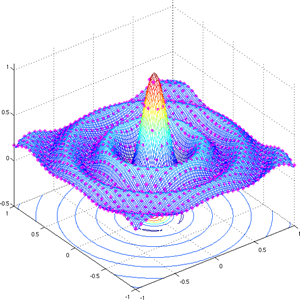
\includegraphics[scale=0.25]{../../img/sinc.PNG}}

\section{前言}
\label{sec:org5fc7108}


在之前的一些博文中,我们提到了概率论中的一些\href{file:///c:/Users/cliyh/AppData/Roaming/zorg/output/computer/MLAPP/MLAPPch2dot3-some-probability-distributions.org}{重要的分布} ;在数学博文中,对这些重要的分布的性质也进行了不同程度的分析。今天,我来简要介绍一下,这些分布在机器学习中的一个应用:共轭先验。

\section{共轭先验}
\label{sec:orgcdeb788}


讨论概率分布的一个重要原因是,现实生活中有很多数据可以使用这些模型来模拟。对于给定的一个数据集合\(x_{1},\ldots ,x_{n}\)我们希望这个数据集合来自于某个随机变量\(X\),并且这个随机变量具有概率分布\(P(X)\)。找到\(P(X)\)的过程叫做密度估计(density estimation)。需要强调的是密度估计问题是一个病态问题,因为世界上的概率密度函数不计其数,能够给出观测集合\(x_{1},\ldots ,x_{n}\)的概率密度函数也是如此之多。任何一个在\(x_{1},\ldots ,x_{n}\)处非零的密度函数\(P(X)\)都可能是候选。选择一个合适的\(P(X)\)是模型选择问题,在机器学习领域经常遇见。

之前我们也看到了很多分布,把这些分布用到密度估计过程中,我们需要确定相对于这些模型的一些重要参数,比如期望,比如方差,再比如一些超参数。这些量值的确定亦有不同的方法,从频率方面(frequentist)着手的话,我们根据某个准则进行优化,为这些参数选择特定的值,常见的准则是最大似然准则。从贝叶斯方面着手的话,我们引入这些参数的一些先验估计(prior distributions),然后使用贝叶斯定理根据给定的观测数据计算关于这些参数的后验估计。 \textbf{这些先验估计的选取非常的关键} 直接影响到参数的准确度和计算的难易程度。常见的做法是选择可能分布的共轭先验。

顾名思义,共轭先验是后验分布的一个先验假设。最重要的, \textbf{共轭先验和后验具有相同的形式} 。这在计算过程中可以非常方便的形成迭代,根据新的观测数据,原先的后验概率变成新的先验概率,继而更新出一个新的后验概率,这个后验概率的参数更加的准确。这个过程大大的简化了贝叶斯分析。举个例子,多变量分布的一个共轭先验叫做狄利克雷分布(Dirichlet distribution),高斯分布的共轭先验是另一个高斯函数。所有的这些函数都是指数函数家族里的分布。
\section{多项分布和狄利克雷分布}
\label{sec:org7eb1fab}


\subsection{多项分布}
\label{sec:orgb360b48}

我们讨论过\href{file:///c:/Users/cliyh/AppData/Roaming/zorg/output/math/probability/binary-distribution.thm}{二项分布} ,对于二项分布的一个扩展就是\href{file:///c:/Users/cliyh/AppData/Roaming/zorg/output/math/probability/afcp-01dot5-multinomial-coefficients.org}{多项分布} 。因为我们经常会碰到一个随机变量的取值是\(K\)个互斥的结果中的一个。尽管有很多方法来描述这个变量,但是我们实用一个\(K\)维的矢量来描述结果会非常容易。举个简单的例子,假设\(K=6\),第三个结果发生,则这个事件可以表示为:
\begin{equation}
\label{eq:1}
\mathbf{x} = (0,0,1,0,0,0)
\end{equation}
任何一个类似这样的矢量都满足:\(sum_{k=1}^{K}x_{k} = 1\),我们用\(\mu_{k}\)来描述\(x_{k}=1\),则\(\mathbf{x}\)的分布可以表示为:
\begin{equation}
\label{eq:2}
p(\mathbf{x}| \mathrm{\mu}) = \prod_{k=1}^{K}\mu_{k}^{x_{k}}
\end{equation}
其中\(\mathbf{\mu} = (\mu_{1},\ldots ,\mu_{K})\)满足\(\mu_{k} \geq 0\),且\(\sum_{k} \mu_{k} = 1\)。很容易想到一个骰子,有六面,假若这个骰子是均匀的则\(\mu_{1} = \ldots = \mu_{6} = 1/6\)。假若这个骰子不均匀,则\(\mu_{k}\)的取值就不一定了,但是依然会满足\(\sum_{k}\mu_{k} = 1\).

现在考虑一个数据集合\(\mathcal{D}\),长度是\(N\),这\(N\)个数来自于对随机变量\(X\)的采样,\(\mathbf{x}_{1},\ldots , \mathbf{x}_{N}\),对应的最大似然函数可以表示为:
\begin{equation}
\label{eq:3}
p(\mathcal{D}| \mathbf{\mu}) = \prod_{n=1}^{N}\prod_{k=1}^{K}\mu_{k}^{x_{nk}} = \prod_{k=1}^{K}\mu_{k}^{(\sum_{n}x_{nk})} = \prod_{k=1}^{K}\mu_{k}^{m_{k}}
\end{equation}
我们看到似然函数只依赖于\(N\)个数据集合的\(K\)个量值:
\begin{equation}
\label{eq:4}
m_{k} = \sum_{n}x_{nk}
\end{equation}
这\(K\)个量值是\(N\)个数据集合的充分统计量。其中\(m_{k}\)表示\(x_{k} = 1\)在\(N\)次观测中出现的总观测次数。

为了找到\(\mathbf{\mu}\)的最大似然解,我们需要最大化\(\ln p( \mathcal{D} | \mathbf{\mu} )\),约束条件是\(\sum_{k} = 1\)。这个过程可以使用拉格朗日乘子算法。
\begin{equation}
\label{eq:5}
\sum_{k=1}^{K}m_{k}\ln \mu_{k}+ \lambda(\sum_{k=1}^{K}\mu_{k} -1)
\end{equation}
对上式针对\(\mu_{k}\)求导,则:
\begin{equation}
\label{eq:6}
\mu_{k} = -m_{k}/\lambda
\end{equation}
把式 (\ref{eq:6})带入拉格朗日乘子的约束条件,我们有\(\lambda = -N\).所以我们得到式\textasciitilde{}(\ref{eq:3})的最大似然解是:
\begin{equation}
\label{eq:7}
\mu_{k}^{ML} = \frac{m_{k}}{N}
\end{equation}
显然这个解是\(N\)次观测过程中\(x_{k}=1\)出现的频次。

基于\(\mathbf{\mu},N\),我们可以考虑量\(m_{1},\ldots ,m_{K}\)的联合分布,则这个分布可以表示为:
\begin{equation}
\label{eq:8}
\mathrm{Mult}(m_{1},m_{2},\ldots ,m_{K}| \mathbf{\mu},N) = \binom{N}{m_{1}m_{2}\ldots m_{K}} \prod_{k=1}^{K}\mu_{k}^{m_{k}}
\end{equation}
式 (\ref{eq:8})叫做多项分布,其中归一化项表示把\(N\)分成\(K\)组的方法,大小为\(m_{1},\ldots ,m_{K}\)。
\begin{equation}
\label{eq:9}
\binom{N}{m_{1}m_{2}\ldots m_{K}} = \frac{N!}{m_{1}!\ldots m_{k}!}
\end{equation}
其中:
\begin{equation}
\label{eq:10}
\sum_{k=1}^{K}m_{k} = N
\end{equation}

\subsection{狄利克雷分布}
\label{sec:orgd8dacef}


在上一节,我们介绍了使用最大似然估计导出多项式分布的方法,这种方法是基于frequestist的。现在我们基于贝叶斯方法,导出多项式分布。

首先我们引入\(\mu_{k}\)的一个先验分布。通过观察多项分布式 (\ref{eq:8}) ,我们发现共轭先验具有如下形式:
\begin{equation}
\label{eq:11}
p( \mathbf{\mu} | \mathbf{\alpha} ) \propto \sum_{k=1}^{K}\mu_{k}^{\alpha_{k} -1}
\end{equation}
其中\(0 \leq \mu \leq 1\) 且\(\sum_{K}\mu_{k} = 1\)。此处\(\alpha_{1},\ldots ,\alpha_{k}\)是分布的参数。由于\(\mu_{k}\)之和为1这个约束的存在,这个关于\(\mu_{k}\)的分布是一个\(K-1\)维的单纯形。

针对式 (\ref{eq:11})的归一化形式,可以表示为:
\begin{equation}
\label{eq:12}
\mathrm{Dir}( \mathbf{\mu} | \mathbf{\alpha} ) = \frac{ \Gamma(\alpha_{0}) }{ \Gamma(\alpha_{1})\ldots \Gamma(\alpha_{K}) } \prod_{k=1}^{K} \mu_{k}^{\alpha_{k} - 1}
\end{equation}
式 (\ref{eq:12})就是狄利克雷分布。这里\(\Gamma(x)\)是伽马函数。 \(\alpha_{0} = \sum_{k=1}^{K}\alpha_{k}\).

把似然函数 (\ref{eq:8}) 和先验函数 (\ref{eq:12}) 相乘,我们得到一个后验分布:
\begin{equation}
\label{eq:13}
p( \mathbf{\mu} | \mathcal{D}, \mathbf{\alpha} ) \propto p( \mathcal{D} | \mathbf{\mu} ) p( \mathbf{\mu} | \mathbf{\alpha} ) \propto \prod_{k=1}^{K} \mu_{k}^{\alpha_{k} + m_{k} -1}
\end{equation}

我们看到后验分布和共轭先验具有相同的形式,他们看起来都像狄利克雷分布。狄利克雷肺部确实是多项分布的共轭先验。
\section{总结}
\label{sec:orgc2749cf}


共轭先验为使用贝叶斯方法提供了有力工具,使得快速迭代变为可能。然而并不是所有的分布都有其共轭先验,所以在具体的案例中还需要具体分析。
\end{document}
